%!TEX program = lualatex
\documentclass[25pt]{tikzposter}
\usepackage[spanish]{babel}
\usepackage{amsmath}
\usepackage[math]{kurier}
\usetheme{Envelope}
%\usebackgroundstyle{Rays}

\definebackgroundstyle{samplebackgroundstyle}{
\draw[inner sep=0pt, line width=0pt, color=white, fill=backgroundcolor!255!black]
(bottomleft) rectangle (topright);
}
\usebackgroundstyle{samplebackgroundstyle}

\geometry{paperwidth=100cm, paperheight=130cm}
\makeatletter
\setlength{\TP@visibletextwidth}{\textwidth-2\TP@innermargin}
\setlength{\TP@visibletextheight}{\textheight-2\TP@innermargin}
\makeatother

%\title{\parbox{\linewidth}{\centering Smart Usage of Context Information for the Analysis, Design, and Generation of Power-Aware Policies for Mobile Sensing Apps}}
\title{\parbox{\linewidth}{\centering Uso inteligente de información contextual para el análisis, diseño y generación de políticas conscientes de la energía para aplicaciones móviles de sensado}}
\author{Rafael Pérez Torres, Dr. César Torres Huitzil, Hiram Galeana Zapién Phd}
\institute{LTI Cinvestav Tamaulipas}
\titlegraphic{
\includegraphics[scale=0.8]{./images/cinvestav-logo-no-text-white}}

\makeatletter
\renewcommand\TP@maketitle{%
   \centering
   \begin{minipage}[b]{0.8\linewidth}
        \centering
        \color{titlefgcolor}
        {\bfseries \Huge \sc \@title \par}
        \vspace*{1em}
        {\Large \@author \par}
        \vspace*{1em}
        {\large \@institute}
    \end{minipage}%
    \tikz[remember picture,overlay]\node[scale=0.8,anchor=east,xshift=-55cm,yshift=6cm,inner sep=0pt] {%
       \@titlegraphic
    };
}
\makeatother

\begin{document}
\node[above right,opacity=0.7,inner sep=0pt,outer sep=0pt] at (bottomleft) {
\includegraphics[width=\paperwidth,height=0.55\paperheight]{images/cinvestav-background.pdf}};
\maketitle
\block{Resumen}{
	Los servicios móviles basados en localización ejecutados por smartphones requieren actualizaciones constantes de ubicación para adaptar su funcionamiento.
	Sin embargo, realizar el seguimiento del usuario mediante proveedores de ubicación clásicos, como el GPS, representa un alto consumo de energía, la cual es un recurso escaso y competido en este tipo de platformas.
	La presente investigación tiene como objetivo reducir el consumo de energía al realizar el seguimiento del usuario, a partir de información contextual que es extraída de datos provenientes de los sensores.
	Dicha información permite al dispositivo aprender sobre los patrones de movilidad del usuario y apoyarse en este conocimiento para realizar un uso adaptativo de los proveedores de ubicación.
}

\begin{columns}
\column{0.25}
\block{Antecedentes (1)}{
\begin{center}
\begin{tikzfigure}
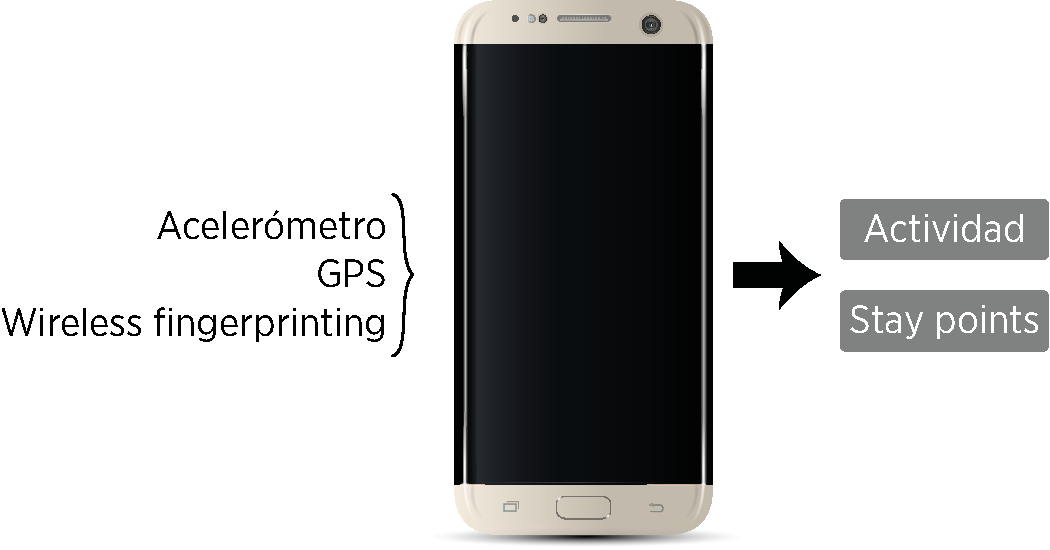
\includegraphics[width=0.12\textwidth]{images/antecedents.pdf}
\end{tikzfigure}  

\begin{itemize}
\item La energía es un recurso limitado en plataformas móviles, como el smartphone.
\item Por ello, el sensado constante (o indiscriminado) no resulta óptimo, descargando rápidamente la batería.
\item Es posible explorar estrategias alternativas para realizar el monitoreo continuo del usuario, atendiendo al compromiso energía-precisión.
\item Tal es el caso del uso de información contextual, la cual permite caracterizar la situación del usuario y emplearla para adaptar de forma dinámica el acceso al GPS.
\end{itemize}
\end{center}
}


\column{0.25}
\block{Problemas (2)}{

\begin{itemize}
\item Dado un conjunto $V = \left\{v_{1}, v_{2}, \dotsc, v_{n}\right\}$ de datos obtenidos del sensor $S$ en el intervalo de tiempo $T  \in [t_{1}, t_{2}]$, identificar el patrón de movilidad actual $p_{S}$ que representa a la actividad del usuario.
\begin{equation}
\fontsize{25}{30}
\selectfont
\text{IdentificadorPatrones}( V ) \longrightarrow{} p_{S} \in \text{Patterns}
\end{equation}
\item Dado el conjunto de patrones de movilidad $\mathcal{P} = \{ p_{S_1}, p_{S_2}, \ldots, p_{S_n} \}$ detectados a partir de datos de los sensores $\mathcal{S} = \{ S_1,S_2,\ldots, S_n \}$, un requisito de precisión $a$, y el estado $c$ de las restricciones del dispositivo móvil, encontrar una política que seleccione el conjunto adecuado de sensores $\mathcal{S}_{new}$ y su configuración asociada $\mathcal{S}_{new_{conf}}$  de tal forma que se cumplan los requisitos de la aplicación.
\begin{equation}
\fontsize{25}{30}
\selectfont
\text{GeneradorPolíticas}( \mathcal{P}, a, c ) \longrightarrow{} \mathcal{S}_{new}, \mathcal{S}_{new_{conf}}
\end{equation}
\end{itemize}
}

\column{0.5}
\block{Hipótesis (3)}{
Es posible utilizar políticas inteligentes generadas a través de información contextual obtenida de datos de los sensores, con el fin de reducir el consumo de energía de un dispositivo móvil al realizar sensado continuo.
}





%\column{0.25}
\block{Objetivos (4)}{

\textbf{Objetivo general:}	Reducir el consumo de energía de aplicaciones móviles de sensado continuo a través de políticas auto-adaptables y conscientes de la energía generadas a partir de información contextual.


\textbf{Objetivos específicos:}
\begin{itemize}
\item Identificar patrones de mobilidad a partir de información contextual obtenida de sensores inerciales (acelerómetro) y proveedores de ubicación (GPS, WPS)
\item Generar políticas para adaptar el uso de sensores a partir de los patrones de movilidad, requisitos de precisión y energía de la aplicación móvil y el estado de las restricciones del dispositivo.
\item Facilitar el desarrollo de aplicaciones móviles de sensado que requieren el seguimiento del usuario, aislando la complejidad del acceso a los sensores y el manejo eficiente de la energía.
\end{itemize}
}
\end{columns}


\begin{columns}
\column{0.5}
\block{Fundamentos de la solución propuesta (5)}{
	\innerblock[linewidth=1pt,roundedcorners=5]{Sistemas dirigidos por eventos (Event-driven systems)}{
		\begin{tikzfigure}
			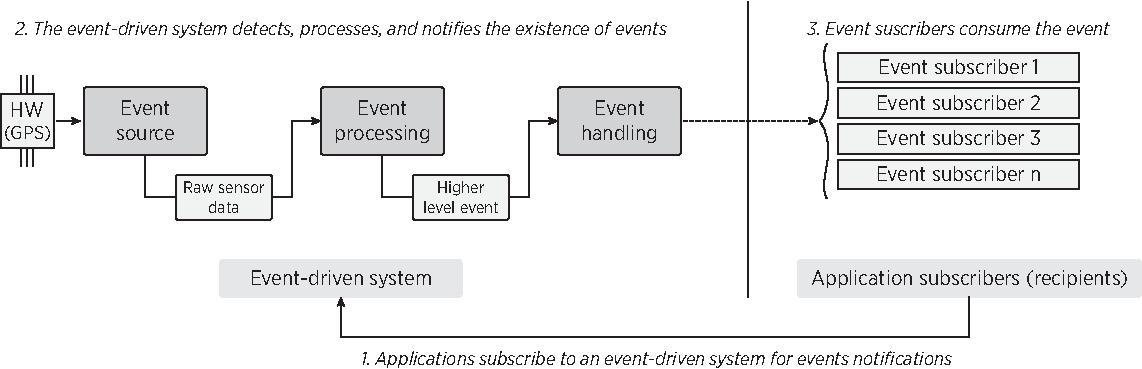
\includegraphics[width=0.32\textwidth]{images/event-driven-system.pdf}
		\end{tikzfigure}
	}
	\vspace{5mm}

	\innerblock[linewidth=1pt,roundedcorners=5]{Movimiento desde la perspectiva de la física (cinemática)}{
	\begin{tikzfigure}[Variaciones de la velocidad de acuerdo a los patrones de movilidad]
			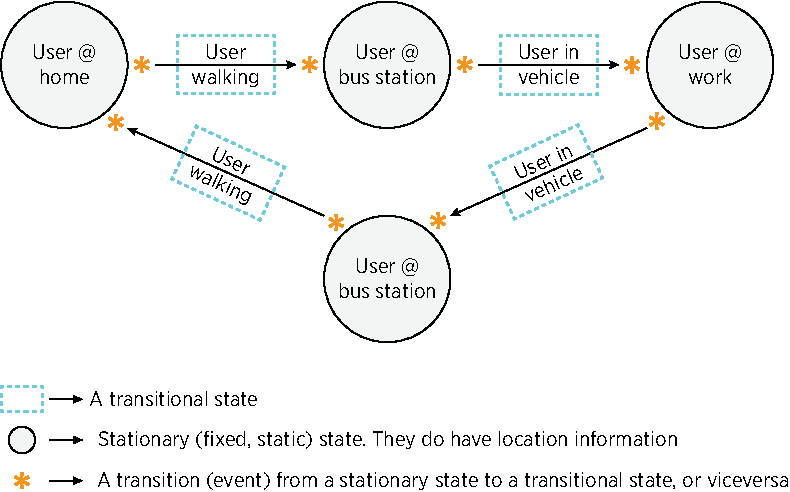
\includegraphics[width=0.23\textwidth]{images/physics-perspective-of-motion}
		\end{tikzfigure}
	}
	\vspace{5mm}

	\innerblock[linewidth=1pt,roundedcorners=5]{Sistemas cognitivos dinámicos}{
	\begin{center}
		\begin{minipage}{0.3\linewidth}
			\begin{itemize}
				\item Percepción
				\item Memoria
				\item Atención
				\item Inteligencia
			\end{itemize}
		\end{minipage}
		%~\hfill
		\begin{minipage}{0.5\linewidth}
			\centering   
				\begin{tikzfigure}
					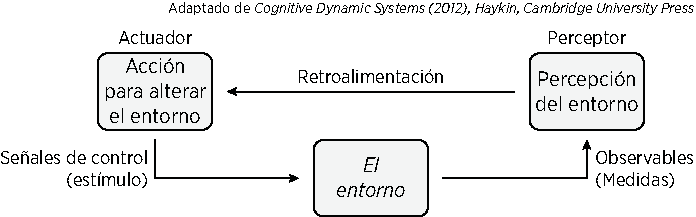
\includegraphics[width=\textwidth]{images/cognitive-dynamic-systems.pdf}
				\end{tikzfigure}
		\end{minipage}
	\end{center}
	}
}


\column{0.5}
\block{Solución Propuesta (6)}{
	\begin{tikzfigure}[Arquitectura de la solución propuesta]
		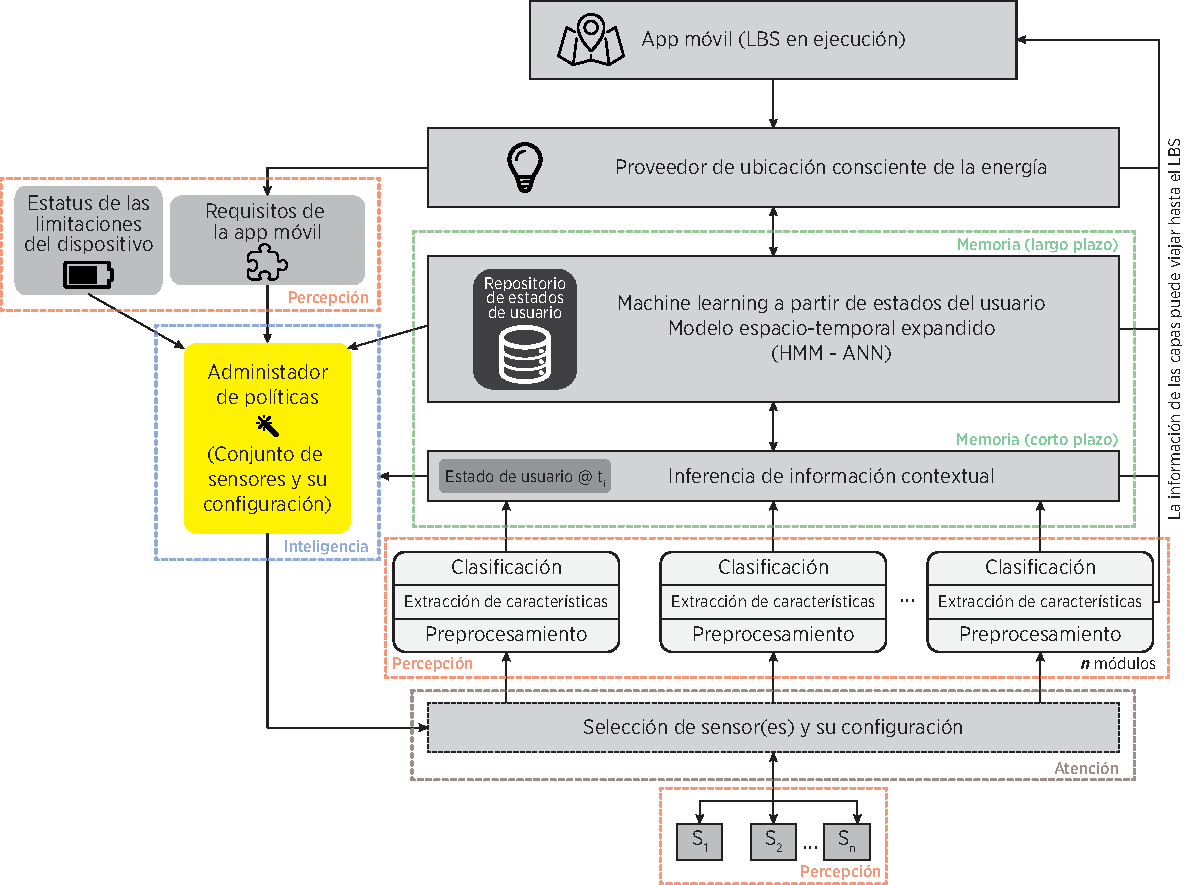
\includegraphics[width=0.28\textwidth]{images/solution-general-overview.pdf}
	\end{tikzfigure}
	\hfill
	\begin{tikzfigure}[Modelo espacio-temporal expandido de la solución propuesta]
		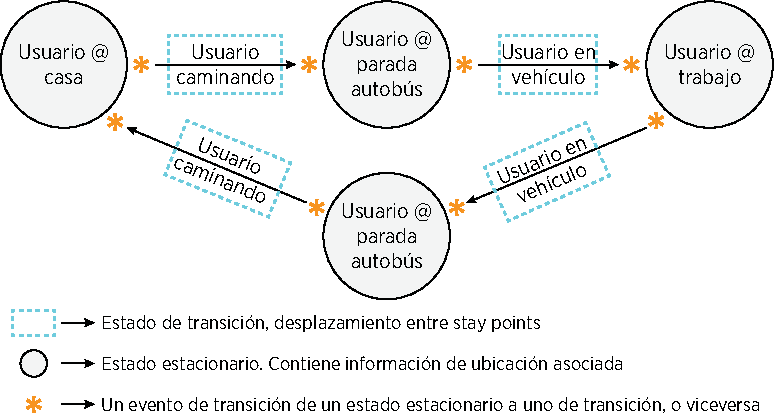
\includegraphics[width=0.16\textwidth]{images/zoom-expanded-spatial-time-model.pdf}
	\end{tikzfigure}
}
\end{columns}

\begin{columns}
\column{0.5}
\block{Resultados preliminares (7)}{
	\begin{center}
		\begin{minipage}{0.65\linewidth}
	  		\centering   
	    	\begin{tikzfigure}[Stay points obtenidos de forma autónoma por el smartphone]
		    	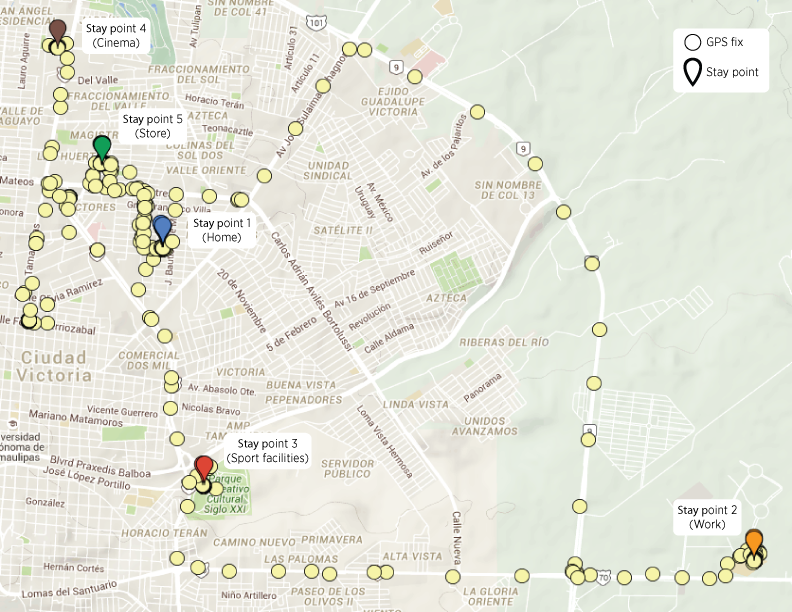
\includegraphics[width=0.34\textwidth]{images/map}
		    	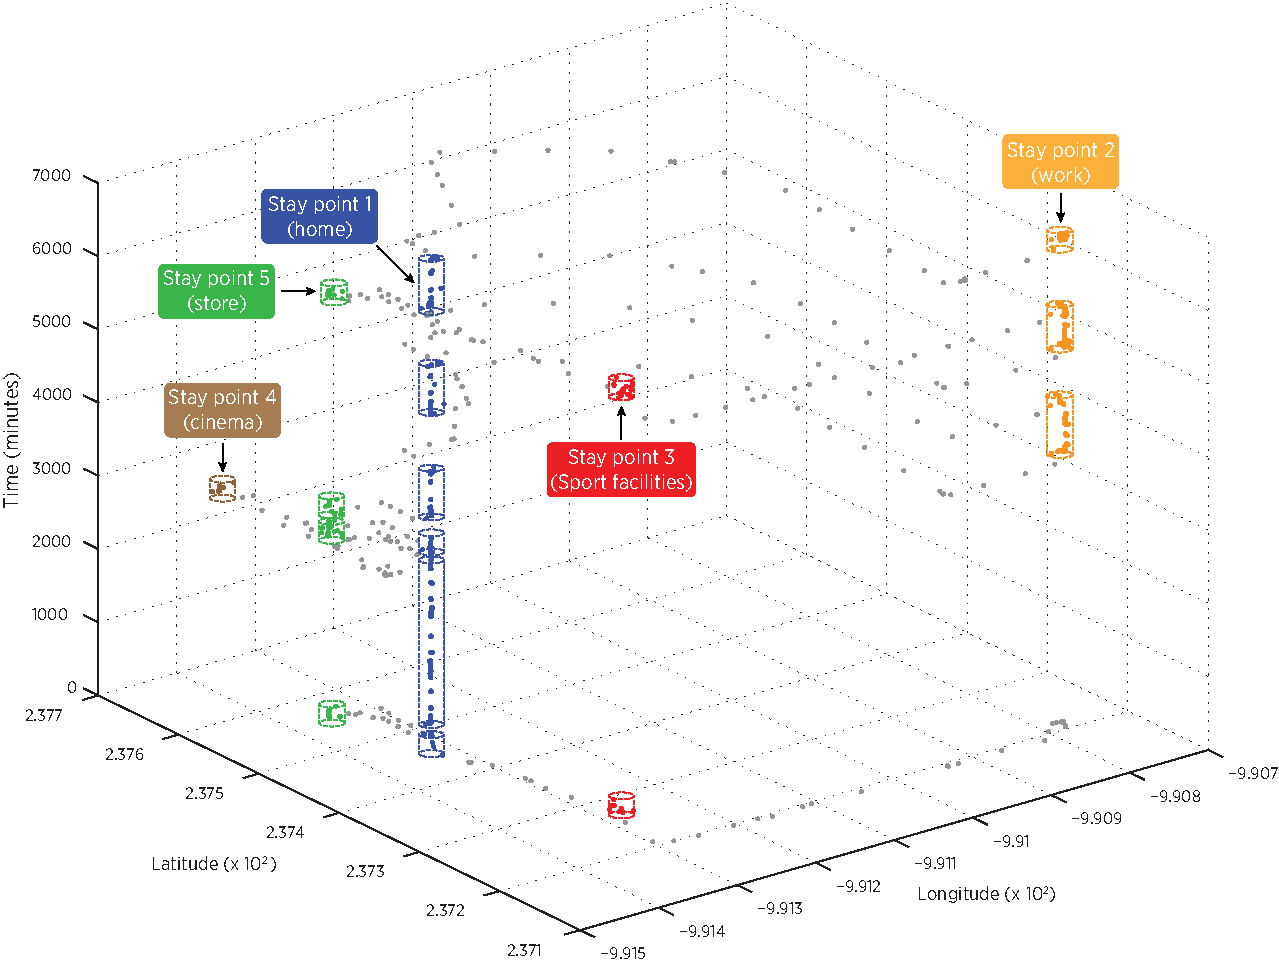
\includegraphics[width=0.34\textwidth]{images/map-three-dimensional}
	    	\end{tikzfigure}
    	\end{minipage}~\hfill
		\begin{minipage}{0.35\linewidth}
			\centering
			\begin{tikzfigure}[Módulo HAR capaz de detectar la actividad física del usuario]
    			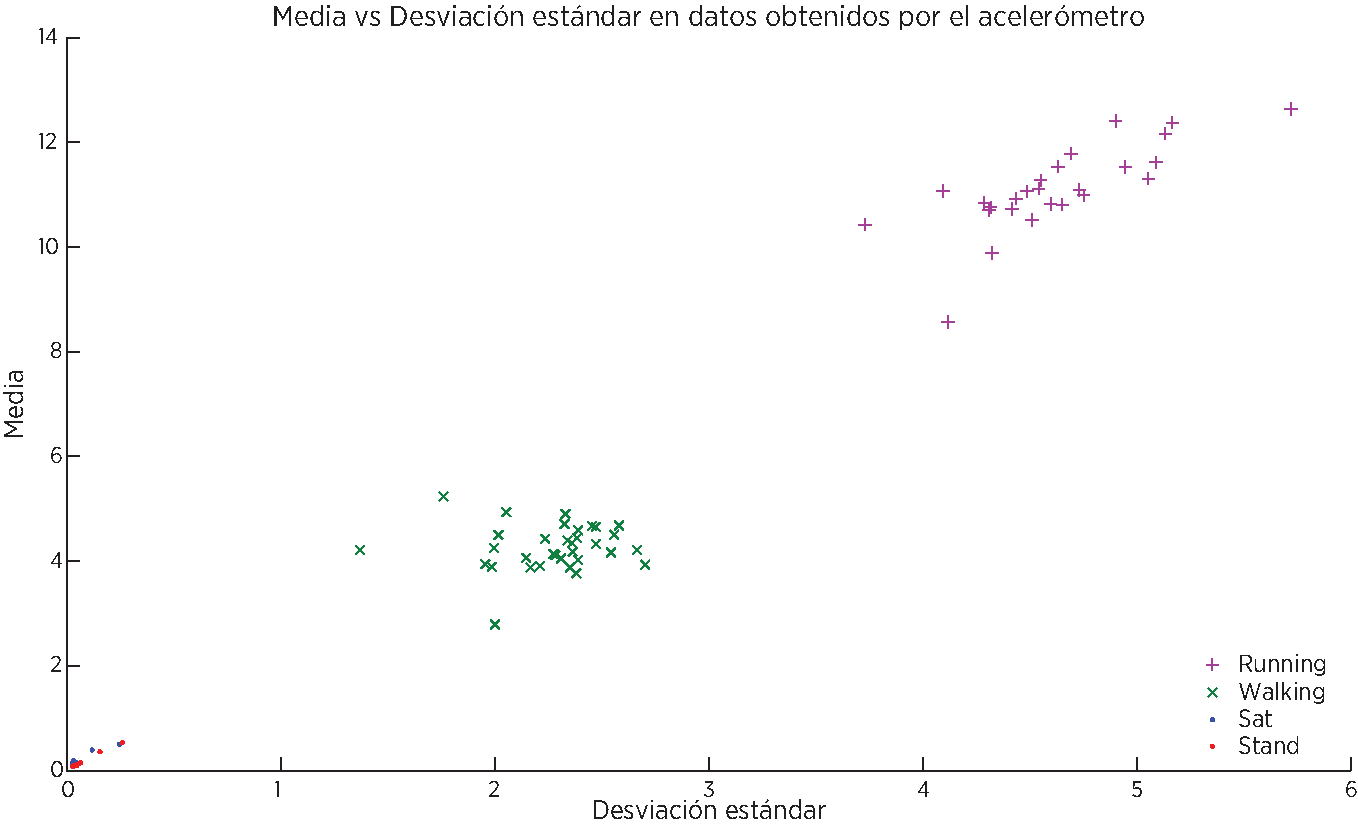
\includegraphics[width=0.8\textwidth]{images/plot-mean-sd.pdf}
			\end{tikzfigure}
		\end{minipage}
	\end{center}
}
\end{columns}

\end{document}